\clearpage
\appendix
\renewcommand{\thetable}{A\arabic{table}}
\renewcommand{\thefigure}{A\arabic{figure}}
\setcounter{table}{0}\setcounter{figure}{0}
\section{Additional results}\label{sec:appendix}

\begin{table}[!h]
\centering
\small
\setlength{\tabcolsep}{3pt}
\caption{Basic properties of the overnight-stay networks, full version}
\label{tab:basic_full}
\resizebox{\linewidth}{!}{\begin{tabular}{lrrrr}
\toprule
 & \shortstack[r]{Ordinary weekday\\13–14 Feb} & \shortstack[r]{Summer holiday\\14–15 Aug} & \shortstack[r]{All Saints\\31 Oct–1 Nov} & \shortstack[r]{Summer, same directed link count\\14–15 Aug} \\
\midrule
\multicolumn{5}{l}{\textit{Size}} \\
\quad People sleeping away from home (millions) & 2.11 & 8.46 & 4.23 & 8.46 \\
\quad Share of them on kept links (\%) & 69 & 83 & 76 & 67 \\
\quad Nodes N (in the giant component) & 2,435 (2,432) & 2,435 (2,435) & 2,435 (2,434) & 2,435 (2,422) \\
\quad Links L (undirected) & 26,465 & 101,996 & 48,698 & 31,573 \\
\quad Density (\%) & 0.89 & 3.44 & 1.64 & 1.07 \\
\addlinespace
\multicolumn{5}{l}{\textit{Degree}} \\
\quad Mean degree $\langle$k$\rangle$ & 21.7 & 83.8 & 40.0 & 25.9 \\
\quad Median degree & 11 & 45 & 22 & 10 \\
\quad Maximum degree $k_{\max}$ (\% of N) & 1,499 (62 \%) & 2,233 (92 \%) & 2,008 (82 \%) & 1,829 (75 \%) \\
\quad Median out-degree / in-degree & 7 / 7 & 14 / 27 & 10 / 16 & 2 / 6 \\
\quad Tail fit, in / out: power law vs log-normal & tie / tie & log-normal / log-normal & tie / tie & log-normal / log-normal \\
\addlinespace
\multicolumn{5}{l}{\textit{Small world}} \\
\quad Average path length $\ell$ (rewired / ER) & 2.44 (2.41 / 2.83) & 2.00 (1.98 / 2.02) & 2.16 (2.11 / 2.49) & 2.25 (2.24 / 2.74) \\
\quad $\ell^*$ = ln N / ln$\langle$k$\rangle$ & 2.53 & 1.76 & 2.11 & 2.39 \\
\quad Diameter (rewired) & 4 (5.1) & 3$^\dagger$ (3.2) & 4$^\dagger$ (4.0) & 4$^\dagger$ (4.9) \\
\quad Clustering $\langle$C$\rangle$ (rewired / ER) & 0.554 (0.247 / 0.009) & 0.546$^\dagger$ (0.387 / 0.034) & 0.593 (0.298 / 0.016) & 0.678 (0.436 / 0.011) \\
\addlinespace
\multicolumn{5}{l}{\textit{Mixing}} \\
\quad Degree assortativity r (rewired) & $-$0.131 ($-$0.140) & $-$0.214 ($-$0.217) & $-$0.155 ($-$0.161) & $-$0.187 ($-$0.186) \\
\quad Range of r reached by rewiring [$r_{\min}$, $r_{\max}$] & [$-$0.221, $-$0.092] & [$-$0.424, $-$0.114] & [$-$0.274, $-$0.098] & [$-$0.271, $-$0.148] \\
\quad Reciprocity (rewired, directed) & 0.52 (0.13) & 0.24 (0.09) & 0.48 (0.15) & 0.24 (0.07) \\
\quad 2nd-order mixing $R_{\mathrm{avg}}$ (null keeping P(k) and $\phi$) & 0.000 ($-$0.023) & $-$0.289 ($-$0.252) & $-$0.129 ($-$0.127) & $-$0.243 ($-$0.191) \\
\addlinespace
\multicolumn{5}{l}{\textit{Rich club and core}} \\
\quad Rich club $\phi$, top 50 zones (rewired) & 0.80 (0.66) & 0.96 (0.92) & 0.91 (0.81) & 0.83$^\dagger$ (0.81) \\
\quad Rich-club clique size (rewired) & 17 (5.8) & 17$^\dagger$ (9.2) & 22 (7.1) & 9$^\dagger$ (7.9) \\
\quad Links touching the top 5 \% of nodes (\%) & 65 & 58 & 63 & 74 \\
\quad Largest k of a non-empty k-core (rewired / ER) & 37 (30 / 15) & 84 (83 / 67) & 51 (45 / 30) & 48 (43 / 18) \\
\bottomrule
\end{tabular}}
\par\smallskip
\begin{minipage}{\linewidth}\footnotesize
One network per night of 2024; a link joins two zones when at least 10 residents of one sleep in the other. Last column: the summer night cut to its 35,812 heaviest links, the size of the ordinary night. In brackets: mean of 50 degree-preserving rewirings (and of 50 Erdős–Rényi graphs where shown). $^\dagger$ The change does not keep its direction on every pair of sister nights.
\end{minipage}
\end{table}


\begin{figure}[t]
\centering
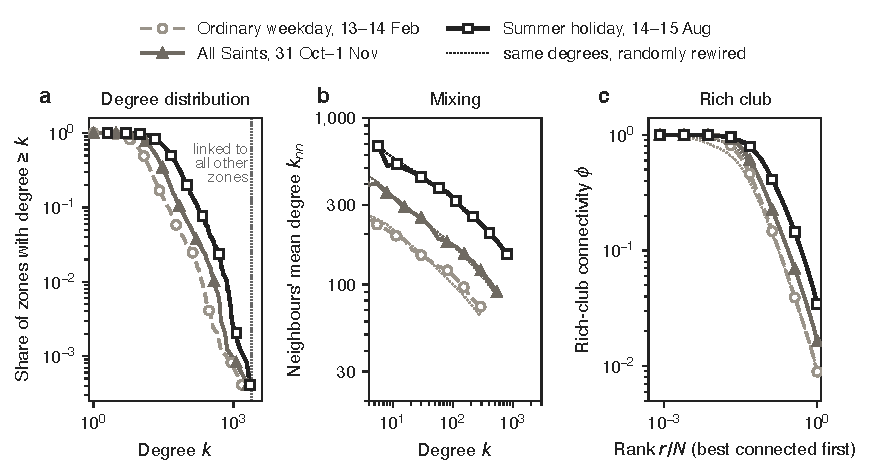
\includegraphics[width=\linewidth]{fig_basic_properties.pdf}
\caption{\textbf{Basic properties of the three networks.} \textbf{a}, Share of zones with degree at least $k$. \textbf{b}, Mean degree of a zone's neighbours, $k_{nn}$, against its degree, in logarithmic bins. \textbf{c}, Rich-club connectivity $\phi$ against the normalised rank $r/N$ of the best-connected zones. Undirected networks with links of at least 10 people; dotted lines show degree-preserving rewired networks (mean of 10 in b and 50 in c).}
\label{fig:basic}
\end{figure}

Figure~\ref{fig:bosam} shows the BOSAM of the three main nights. On every night the dark band along the top and the right edge shows the same pattern: zones of every degree link mainly to a few best-connected zones, Madrid last in the order. The visible change on holiday nights is density (3.4\,\% of pairs linked in summer against 0.9\,\% on the ordinary night). The 121 best-connected zones are linked in 44\,\%, 59\,\% and 78\,\% of their pairs on the ordinary, All Saints and summer nights; degree-preserving rewiring gives 38\,\%, 55\,\% and 76\,\%. The self-similar envelope test of \citet{guo2009fingerprint} is not informative here, because Madrid is the largest-index neighbour of 62--92\,\% of zones, so most leaf envelopes end on its row. The BOSAM ignores the direction of links, so the split into senders and receivers (Figure~\ref{fig:senders}) does not show in it.

\begin{figure}[t]
\centering
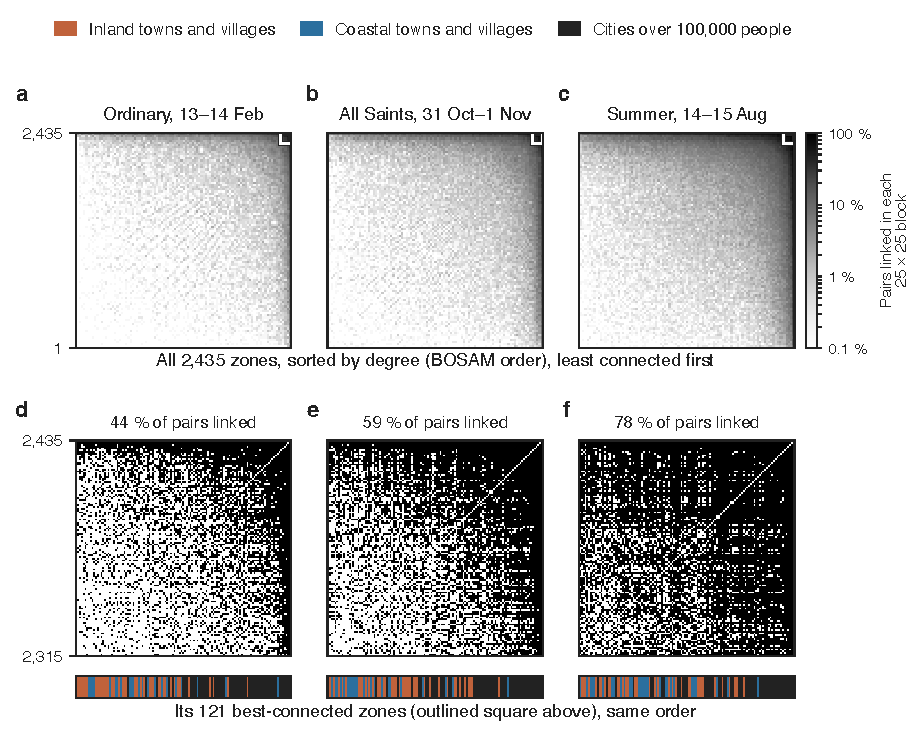
\includegraphics[width=\linewidth]{fig_bosam.pdf}
\caption{\textbf{Bitmap of the sorted adjacency matrix (BOSAM) of the three nights.} \textbf{a--c}, The matrix, zones sorted by degree as in \citet{guo2009fingerprint}; the grey level is the share of linked pairs in blocks of $25\times25$ zones, on one logarithmic scale; the 10 least connected zones, which do not fill a block, are not drawn. \textbf{d--f}, The 121 best-connected zones (outlined square in a--c), one cell per pair; the strip gives the kind of zone. Undirected networks with links of at least 10 people.}
\label{fig:bosam}
\end{figure}

\begin{table}[t]
\centering
\small
\caption{Change in the pull of the roots, 14--15 August minus 13--14 February, under different treatments of empty city--province cells}
\label{tab:zero}
\begin{tabular}{lrrr}
\toprule
Treatment & Arrived before 1981 & Arrived 2016--2023 & Born in a village \\
\midrule
Add 0.5 to each count (main) & $+0.084$ & $-0.072$ & $+0.086$ \\
Add 1 to each count & $+0.113$ & $-0.097$ & $+0.100$ \\
Add 0.1 to each count & $+0.038$ & $-0.036$ & $+0.045$ \\
Add $10^{-4}$ to each share & $+0.059$ & $-0.051$ & $+0.091$ \\
Add $10^{-5}$ to each share & $+0.017$$^{\circ}$ & $-0.019$$^{\circ}$ & $+0.028$ \\
$\operatorname{asinh}(1000\times\text{share})$ & $+0.141$ & $-0.120$ & $+0.202$ \\
112 large cities, 22 provinces & $+0.082$ & $-0.135$ & $+0.098$ \\
\bottomrule
\end{tabular}
\par\smallskip
\begin{minipage}{\linewidth}\footnotesize
All destinations; groups entered together as in Figure~\ref{fig:roots}. Between 46\,\% and 60\,\% of city--province cells have no sampled resident of a group, so the regressor needs a rule for empty cells. $^{\circ}$\,Wild cluster bootstrap $p\geq0.05$. Source: results/v1\_c1\_zero\_sensitivity.csv.
\end{minipage}
\end{table}


Table~\ref{tab:zero} repeats the generation contrasts of Figure~\ref{fig:roots} under six rules for empty city--province cells, and on the 112 large cities of the full census table, where few cells are empty. The sign never changes: the pre-1981 group and the village-born always pull harder in August and recent arrivals always pull less. The size does change, from $+0.017$ to $+0.141$ for the pre-1981 group, and with the smallest constant two of the three contrasts are no longer significant. This is why the text reports signs and intervals for the main rule but does not compare sizes across groups or nights.
